\documentclass[11pt]{article}
\usepackage[margin=1.1in]{geometry}
\usepackage{amsmath,amssymb}
\usepackage{graphicx}
\usepackage{booktabs}
\usepackage{microtype}
\usepackage[hidelinks]{hyperref}
\usepackage{xcolor}
\usepackage[numbers,sort&compress]{natbib}

\newcommand{\eps}{\varepsilon}
\newcommand{\betadep}{\beta_{\mathrm{dep}}}
\newcommand{\betaimp}{\beta_{\mathrm{imp}}}
\newcommand{\kk}{\langle k^{2}\rangle/\langle k\rangle}

\title{Proofs after AlephZero:\\ dependency networks, belief dynamics, and the structure of
AI-era mathematics\\[0.6em]\large --- draft ---}
\author{}
\date{August 1, 2026}

\begin{document}
\maketitle

\begin{abstract}
Viteri and DeDeo (2022) showed that mathematical proofs, viewed as networks of claims and
deductive dependencies, share a characteristic topology---heavy-tailed reuse of claims with
exponent $\alpha\!\approx\!2$ and strong modularity---and that a simple asymmetric-Ising model of
belief propagation on these networks undergoes epistemic phase transitions (EPTs): sharp
collective jumps to near-certainty despite noisy inference. We extend this analysis to the
mathematics humans and machines have produced together since: four Lean 4 megaprojects
(Polynomial Freiman--Ruzsa, Fermat's Last Theorem, sphere packing in dimension~8 in human-led and
AI-completed versions, and the Equational Theories Project), three generations of AI provers
(AlphaProof 2024, Gauss 2026, AlphaProof Nexus 2026), and a matched human-vs-ATP corpus of 1{,}274
Mizar theorems. We extract dependency networks at three grains---informal blueprint, textual
Lean source, and the compiled kernel environment, which serves as ground truth---and validate the
textual grain against the kernel (precision $0.77$--$0.92$). Five findings. (1)~Heavy-tailed
reuse ($\alpha\!\approx\!2$--$3$) appears in every \emph{constructed} corpus, human or agentic-AI,
at every grain; informal blueprints instead show the hub-deficient ``Wiles signature''
($\alpha\!\approx\!3.3$--$4.6$). (2)~Search-generated proof corpora are structurally different:
the Equational Theories machine stratum is certificate dust, and---controlling for the task's
parallelizability---automated provers on the general Mizar library find proofs that are
three times leaner, $71\%$ rerouted off the human premise set, and hub-poor. Methods sort
instances by depth: search operates where dust suffices, and every deep instance was solved by
construction. (3)~Null models and a parametric $\alpha$-sweep decompose the model's
phenomenology: belief onset is a degree-sequence phenomenon tracking $\kk$, modular firewalls are
a modularity phenomenon, and the genuinely transition-like structure on finite proof networks is
bistability---belief and disbelief are both self-sustaining, with the prior selecting the basin.
(4)~In the paper's asymmetric model, backward refutation is gated by redundancy: reuse hubs are
refutation-proof at any coupling ratio, while single-consequence links transmit doubt once
abduction dominates. (5)~AI provers converged on the human epistemic architecture in about two
years, overshooting human claim-naming density threefold. We interpret these results as evidence
that the 2022 signature is the fingerprint of bounded-context construction---of any prover that
must build on its own past work---and that search-based proving creates a new stratum of
verified mathematics that does not participate in the reuse economy on which, per the model,
mathematical belief is built.
\end{abstract}

\section{Introduction}

How does a community come to \emph{believe} a proof? The standard picture---each step checked,
certainty accumulating multiplicatively---fails on its own terms: a thousand-step proof checked
with per-step reliability $0.99$ would command negligible credence, yet mathematicians are
(correctly) far more confident than Hume's paradox allows. Viteri and DeDeo~\cite{viteri2022}
proposed a structural resolution. Treating a proof as a directed network of claims (nodes) and
deductive dependencies (edges), they found across corpora from Euclid to Coq a characteristic
topology: the number of later claims that reuse a given claim follows a heavy-tailed distribution
with exponent $\alpha \approx 2$, organized into modules. On such networks, a simple model of
noisy belief propagation---an asymmetric Ising model in which belief in a claim couples forward
to its premises and backward to its consequences---exhibits \emph{epistemic phase transitions}:
below a critical inference-error rate, belief crystallizes collectively to near-certainty,
sustained not by any single chain but by the redundancy of the whole. The same structure
quarantines local doubt inside modules (``firewalls''). One outlier proved suggestive: the
network of Wiles's proof of Fermat's Last Theorem, reconstructed from the published text, showed
a hub-deficient $\alpha \approx 3.4$---a possible signature of communication-grain mathematics,
as against the verification grain.

That paper analyzed mathematics written by humans for humans, occasionally with proof
assistants. The four years since have produced something new: mathematics written by humans and
machines \emph{together}, at scale, in styles ranging from carefully blueprinted formalization
collaborations to reinforcement-learning provers to fully automated first-order search. This
paper asks what happened to the 2022 signature in that transition---and uses the new corpora,
which come with compiled ground truth, to put the original claims under substantially sharper
tests than were possible before.

Two companion theoretical works frame the questions. DeDeo and Duede's correspondence
problem~\cite{dedeo2026} asks when a formal artifact \emph{tracks} the informal mathematics it
allegedly formalizes---a condition we operationalize and measure. DeDeo's
AlephZero essay~\cite{dedeo2024} asks what happens to mathematical experience when machines
produce verified results that no human mind has assimilated; the Equational Theories machine
stratum turns out to be a clean empirical instance.

Concretely, we make five contributions. First, a three-grain extraction pipeline (informal
blueprint, textual Lean, compiled kernel) applied to four Lean megaprojects, with the kernel
grain---obtained by loading compiled environments and reading each constant's actual proof-term
dependencies---serving as ground truth against which the textual grain is validated. Second,
measurements of the reuse topology across human, agentic-AI, and search-generated corpora,
including a matched human-vs-ATP comparison on the general Mizar library that controls for the
confound that some tasks are simply parallel. Third, a causal decomposition of the belief
model's phenomenology via degree- and modularity-controlled null models and a parametric
$\alpha$ sweep, together with sharper tests of what ``phase transition'' can mean on a finite
proof network. Fourth, an analysis of the paper's asymmetric model over its full
$(\betadep,\betaimp)$ plane, including the Lakatosian mechanism of backward refutation. Fifth,
a longitudinal analysis of AI proof style, 2024--2026. Throughout, we report the results of five
adversarial audit rounds, including two claims that were corrected under audit; the corrections
are stated in place.

\section{Data and the three grains}
\label{sec:data}

\paragraph{Corpora.} We analyze four Lean~4 formalization megaprojects, pinned at commits of
July~31, 2026: \textbf{PFR} (Tao et al.'s formalization of the polynomial Freiman--Ruzsa
conjecture; the 2023 project generally credited with establishing the blueprint-driven
collaboration model); \textbf{FLT} (Buzzard et al.'s ongoing formalization of Fermat's Last
Theorem); \textbf{Sphere} (the human-led formalization of Viazovska's sphere-packing theorem in
dimension~8) and \textbf{Gauss-Sphere} (Math~Inc.'s completion of the same blueprint by the
agentic AI system Gauss, including a machine-formalized dimension-24 subtree); and \textbf{ET}
(the Equational Theories Project: Tao et al.'s crowdsourced-plus-automated settlement of all
$22{,}028{,}942$ implications among 4{,}694 equational laws of magmas). For AI proof style we
use AlphaProof's 2024 IMO solutions, the corresponding human formalizations from
\texttt{compfiles}, and AlphaProof Nexus's 2026 outputs. For the human-vs-ATP comparison we use
the Mizar40 dataset (premises used in minimized Vampire/E proofs of 32{,}524 Mizar
theorems~\cite{kaliszyk2015}) crossed with MPTP2078 (human Mizar proof
dependencies~\cite{alama2014}).

\paragraph{Grains.} Each Lean project yields up to three networks. The \emph{blueprint grain}
parses the project's \texttt{leanblueprint} LaTeX: nodes are labeled statements; edges are the
author-declared \verb|\uses{}| dependencies; \verb|\lean{}| tags link nodes to formal
declarations and \verb|\leanok| flags record completion status. This is mathematics as
communicated. The \emph{textual grain} parses Lean sources directly: nodes are named
declarations, edges are name references in statement or proof text (namespace-aware; matching
rules audited as described in \S\ref{sec:audit}). The \emph{kernel grain} is ground truth: we
build each project, load the compiled environment, and record for every project constant the
constants actually used by its type and its proof term
(\texttt{Expr.getUsedConstants}).\footnote{Two implementation facts matter for reproduction
under Lean 4.33's module system: private \texttt{.olean} parts load only for modules imported
with per-module \texttt{importAll := true}, and theorem proof terms are returned by
\texttt{ConstantInfo.value?} only with \texttt{allowOpaque := true}.} Edges point from used to
user; out-degree of a node is therefore the number of later results that reuse it.

\begin{table}[t]
\centering
\small
\begin{tabular}{lrrrrr}
\toprule
project & kernel $N$ / $E$ & kernel $\alpha$ & textual $\alpha$ & text.\ prec./rec. & tracking (kernel) \\
\midrule
PFR & 1{,}304 / 5{,}607 & $2.46 \pm 0.23$ & $2.52 \pm 0.28$ & $0.92$ / $0.52$ & $86\%$ \\
FLT & 4{,}723 / 17{,}147 & $2.99 \pm 0.29$ & $2.47 \pm 0.22$ & $0.77$ / $0.52$ & $79\%$ \\
Sphere (human) & 1{,}483 / 4{,}535 & $2.49 \pm 0.19$ & $2.97 \pm 0.40$ & $0.92$ / $0.56$ & $66\%$ \\
Sphere (Gauss) & 5{,}452 / 20{,}739 & $2.56 \pm 0.12$ & $2.51 \pm 0.11$ & $0.88$ / $0.59$ & --- \\
ET & 48{,}505 / 336{,}491 & $2.88 \pm 0.07$ & $2.14 \pm 0.10$ & $0.905$ / $0.60$ & $43\%$ \\
\bottomrule
\end{tabular}
\caption{Kernel-grain networks and validation of the textual grain against them. Precision and
recall are computed on shared declarations. Tracking fidelity is the fraction of blueprint edges
realized as kernel dependency paths of length $\le 6$ between \texttt{\textbackslash lean}-tagged
declarations (\S\ref{sec:tracking}).}
\label{tab:kernel}
\end{table}

\paragraph{Validation.} Table~\ref{tab:kernel} compares grains. The textual grain is a
high-precision subsample of the kernel truth ($0.77$--$0.92$ precision) with roughly half recall;
the missing edges are dominated by elaboration-mediated uses (instance resolution, notation,
tactic-internal lemmas), and $68$--$87\%$ of missed edges point into \emph{definitions} rather
than theorems. Network-level statistics agree between grains within errors on every project,
which is itself evidence that both extractors are sound. All cross-corpus comparisons below use
matched grains.

\section{The reuse topology of constructed mathematics}
\label{sec:alpha}

\begin{figure}[t]
\centering
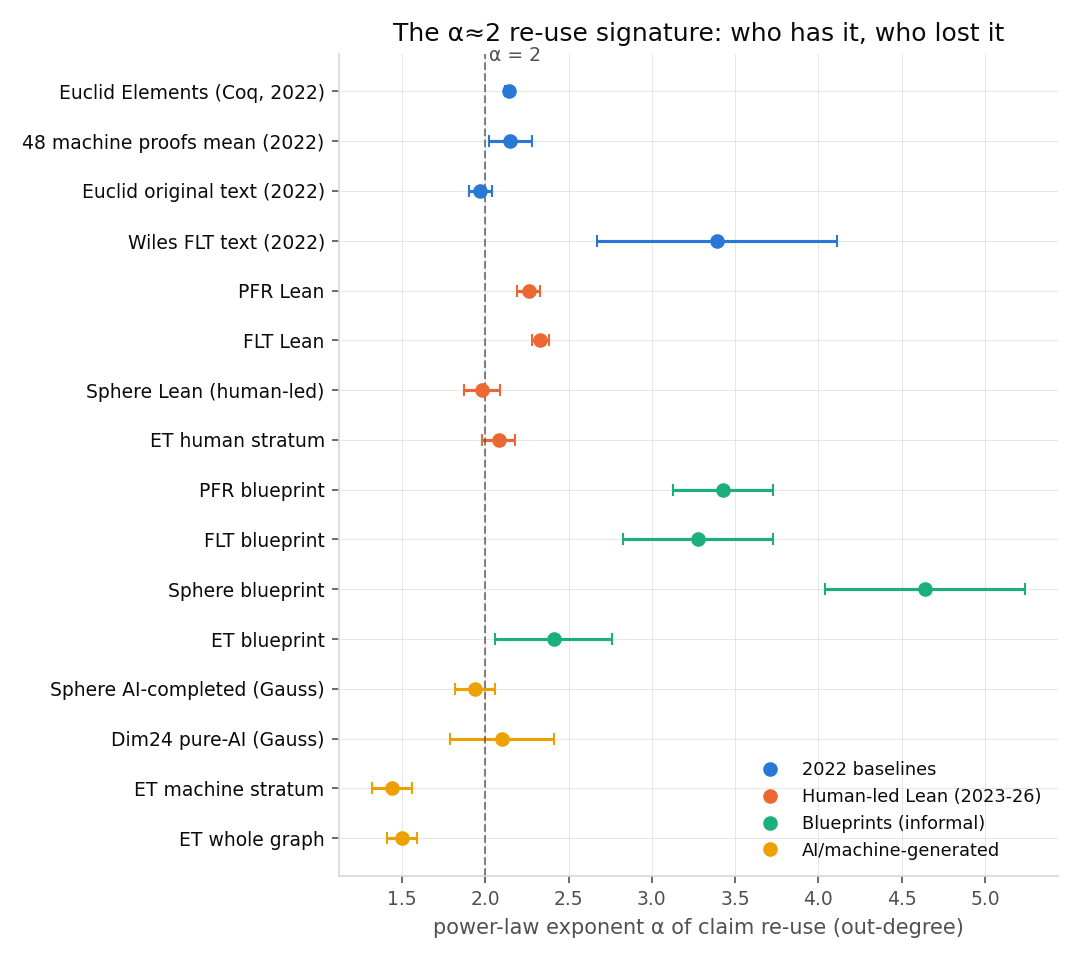
\includegraphics[width=0.8\textwidth]{../figs/f3_alpha_light.png}
\caption{Reuse exponents across corpora and grains. Constructed corpora---human-led Lean,
agentic-AI Lean, and their compiled kernels---cluster in the heavy-tailed
$\alpha\!\approx\!2$--$3$ band of the 2022 baselines; informal blueprints sit apart at
$\alpha\!\approx\!3.3$--$4.6$ (the Wiles signature).}
\label{fig:alpha}
\end{figure}

Fitting discrete power laws by the Clauset--Shalizi--Newman procedure~\cite{clauset2009}
(maximum likelihood with KS-optimal $x_{\min}$), every constructed corpus lands in the same
band (Fig.~\ref{fig:alpha}): human-led Lean projects at $\alpha = 2.47$--$2.97$, the ET human
stratum at $2.52 \pm 0.17$, Gauss's AI-completed corpus at $2.51 \pm 0.11$ (its pure-AI
dimension-24 subtree: $2.55 \pm 0.14$), and the kernel ground truths at $2.46$--$2.99$. The
hubs are the reused workhorses one would name by hand: in PFR, Ruzsa distance and the entropy
toolbox; in ET, the \texttt{Magma} structure itself (reused $34{,}032$ times at kernel grain).

\paragraph{What ``$\alpha \approx 2$'' can and cannot mean.} Under audit, the distributional
claim requires care. A Vuong likelihood-ratio test cannot distinguish power law from lognormal
on the four smaller kernel tails ($|R| < 1.96$); the CSN goodness-of-fit bootstrap does not
reject the power law for PFR/FLT/Sphere/Gauss ($p = 0.15$--$0.85$) but \emph{rejects} it for ET
($p < 0.01$), the one corpus whose tail ($n_{\text{tail}} = 665$) gives the test power. At a
common fixed $x_{\min} = 8$ all five corpora sit tightly in $\alpha = 2.1$--$2.6$. We therefore
state the finding as: \emph{heavy-tailed, approximately power-law reuse with hubs}, robust
across corpora and grains---with the strict power-law form failing exactly where the data can
test it. Module-jackknife shows PFR's tail leans on its entropy library (drop-one-module range
$[2.0, 4.3]$); the Gauss corpus is the most homogeneous ($[2.55, 2.66]$).

\paragraph{The Wiles signature is a communication-grain property.} Within the same projects,
the blueprint networks show $\alpha = 3.43 \pm 0.54$ (PFR), $3.28 \pm 0.72$ (FLT),
$4.64 \pm 1.15$ (Sphere), $2.41 \pm 0.31$ (ET)---the hub-deficit that the 2022 paper found in
the Wiles text. This is not a granularity artifact: contracting the Lean graphs to file level,
matching blueprint size ($N = 58$--$215$), leaves $\alpha$ at $2.1$--$3.0$. At matched scale,
formal mathematics keeps its hubs; the mathematics written for humans does not. Mathematics as
communicated and mathematics as verified have measurably different topology, inside the same
projects, written by the same people.

\section{Machine-generated mathematics: dust, depth, and rerouting}
\label{sec:machine}

\subsection{The Equational Theories machine stratum}

ET's \texttt{Generated/} stratum---24{,}393 kernel declarations produced by simple rewriting,
finite-model search, Vampire, and brute force---is structurally unlike everything else in this
paper. At the textual grain, $95\%$ of machine declarations have no internal edges at all
(12{,}298 disconnected components); the four largest generation methods have exactly zero. At
the kernel grain the apparent internal edges resolve, on inspection, into auto-generated
restatement pairs (\texttt{Law$_X$\_implies\_Law$_Y$} wrapping
\texttt{Equation$_X$\_implies\_Equation$_Y$}): there is no genuine certificate-to-certificate
reuse outside the human-designed Greedy framework. Dependency between strata is one-way:
$200{,}614$ kernel edges flow human$\to$machine; $37$ flow back. We read all 37: they are
genuine (25 support the Sheffer-algebra development; the human \texttt{Tarski543} proof chains
nine machine certificates in sequence)---so the accurate statement is that $0.15\%$ of
certificates have ever been reused by a human proof.

\subsection{The parallel-task confound, and what survives it}
\label{sec:confound}

An objection (raised against an earlier draft of this analysis): the magma
implication problem was \emph{selected} for parallelizability---most of its $2.2\times10^{7}$
instances are independent shallow checks---so certificate dust may reflect the task, not the
prover. The objection is half right, and testing it sharpened the claim.

Define a result's \emph{construction-specific support} as the size of its transitive dependency
closure at kernel grain, excluding equation definitions and mass-cited framework (declarations
cited by $>300$ results). Human-authored \emph{ordinary} implications (213 of them) have median
support $1$---statistically identical to the machine-search certificates. On the easy mass of
the task, humans build no intermediate structure either; that flatness is the task's. But the
same task contains deep instances, and there the split is by method: the 34 human
counterexample results (\texttt{Facts} batches, including the Equation-1692 and Equation-1729
constructions) carry median support $33$ (max $53$); the 1{,}078 machine \texttt{Facts} carry
uniformly $\le 2$ (a stamped finite-table template); the Greedy method---a human-designed
framework machine-instantiated per equation---sits between (tail to $31$). Every deep instance
that was solved was solved by construction. The refined claim: \emph{search does not destroy
structure; it operates exactly where dust suffices, and methods sort instances by depth.}

\subsection{Search on a general library: the Mizar comparison}
\label{sec:mizar}

The confound demands a corpus of search-generated proofs on mathematics \emph{not} selected for
parallelizability. The Mizar40 experiments~\cite{kaliszyk2015} had Vampire/E re-prove
32{,}524 theorems of the general Mizar Mathematical Library, recording the premises used by
each minimized ATP proof; MPTP2078~\cite{alama2014} encodes the human Mizar proof dependencies
for 2{,}078 theorems on the track to Bolzano--Weierstrass. Their intersection gives 1{,}274
theorems of ordinary mathematics---topology, analysis, set theory---each with both a human and
a search-found proof of the \emph{same statement} over the same library.

After removing MPTP background axioms (present in $>30\%$ of problems), three differences
(Table~\ref{tab:mizar}). ATP proofs are three times leaner (5.1 vs.\ 16.5 premises). They are
heavily \emph{rerouted}: only $29\%$ of the premises an ATP proof uses appear in the human
proof's dependency set. And the reuse economy differs in the predicted direction: human premise
usage across the corpus is hub-concentrated ($\alpha = 2.36 \pm 0.09$ on a 248-premise tail;
Gini $0.740$), ATP usage flatter and hub-poor ($\alpha = 3.18 \pm 0.38$ on a 33-premise tail;
Gini $0.567$). A size-matched control (human dependency lists subsampled to ATP proof sizes,
20 replicates) leaves human Gini at $0.669 \pm 0.002$, still well above the ATP: the
concentration gap is not a proof-length artifact. Two caveats cut opposite ways: Mizar40's
premise selection was $k$-NN-trained on human proofs, biasing the ATP \emph{toward} human
routes; ATP proof minimization may prune genuinely-used context. The conclusion: even where
search succeeds on ordinary mathematics, it finds valid proofs that avoid the canonical toolbox
human proofs concentrate on, and it does not reproduce the concentrated reuse economy.

\begin{table}[t]
\centering
\small
\begin{tabular}{lrrrrr}
\toprule
 & premises/proof & distinct premises & reuse $\alpha$ & Gini & in human dep.\ set \\
\midrule
human (Mizar) & 16.5 & 2{,}065 & $2.36 \pm 0.09$ & 0.740 & --- \\
human, size-matched & 5.1 & --- & --- & $0.669 \pm 0.002$ & --- \\
ATP (Vampire/E) & 5.1 & 1{,}789 & $3.18 \pm 0.38$ & 0.567 & $29\%$ \\
\bottomrule
\end{tabular}
\caption{Premise-usage networks over the same 1{,}274 general-library theorems.}
\label{tab:mizar}
\end{table}

\section{Belief dynamics: what causes what}
\label{sec:ising}

We replicate the 2022 model exactly: claims are spins $s_i = \pm 1$; Glauber dynamics with
field $h_i = \betadep \sum_{j \in \mathrm{dep}(i)} s_j + \betaimp \sum_{k \in \mathrm{imp}(i)} s_k$;
coupling related to a per-step inference error rate by $\eps = 1/(1 + e^{2\beta})$; initial
belief $p_{\mathrm{prior}} = 0.75$. On every connected network in our corpus---including the
Gauss corpus and the kernel ground truths---mean belief rises to near-unity at low $\eps$
with modular firewalls $\Delta L_1 \approx +3$ to $+14$, reproducing the 2022 phenomenology on
AI-era data. The new corpora, however, permit sharper questions: \emph{which} structural
property causes \emph{which} phenomenon?

\subsection{Null models and the causal $\alpha$ arm}

Holding the real PFR kernel degree sequence fixed while destroying other structure
(within-module rewiring, global configuration-model rewiring, DAG-respecting rematching), the
belief curve is reproduced essentially exactly in every case; the $\Delta L_1$ firewall instead
collapses from $\approx\!+11$ to $\approx\!+6$ precisely when modularity is destroyed, and is
indifferent to everything else. Acyclicity matters for neither. The decomposition replicates on
FLT. \emph{The belief curve is a degree-sequence phenomenon; the firewall is a modularity
phenomenon.}

The converse experiment dials $\alpha$ directly: synthetic directed graphs at matched size and
density with out-degree tails $\alpha \in \{1.8, 2.2, 2.6, 3.2, 4.0\}$ plus a Poisson control.
Belief onset moves monotonically with tail weight---$\eps_c = 0.43$ at $\alpha = 1.8$ down to
$0.24$ at $\alpha = 4.0$---tracking the mean-field prediction that the critical coupling scales
as $\langle k \rangle / \langle k^2 \rangle$~\cite{dorogovtsev2002}; the Poisson control falls
on the same $\kk$ curve. $\alpha$ causally sets where collective certainty becomes possible,
through degree fluctuations.

\subsection{Is it actually a phase transition?}
\label{sec:transition}

Three tests replace eyeball criteria, and one earlier claim of ours did not survive them. On
the real PFR network the susceptibility $\chi(\eps) = N \,\mathrm{Var}(m)$ shows \emph{no
interior peak} on $\eps \in [0.10, 0.46]$: the smooth belief curve is a finite-size crossover,
and crossover midpoints (``$\eps_c = 0.33$'') should be read as such. What is sharply present is
\emph{bistability}: initialized all-believing versus all-doubting, the network reaches different
locked states at every tested $\eps \le 0.46$ (hysteresis gap $0.66$ even there). On a finite
proof network at realistic error rates, the genuinely transition-like structure is this memory:
belief and disbelief are both self-sustaining collective states, and the prior decides the
basin. Maximum curve slope grows with network size ($3.0 \to 5.1$ across subsamples from
$N = 225$ to $23{,}000$), consistent with a true singularity in the large-$N$ limit, though
subsampling distorts degree structure enough that we hold this loosely.

The corrected claim: an earlier version of this analysis, computed on a grid truncated at
$\eps \le 0.40$, reported that an Erd\H{o}s--R\'enyi control ``blurs'' the transition. Extending
the grid shows the opposite: ER has a \emph{sharper}, classic collective transition at
$\eps \approx 0.44$, fully disordered above it. The real network instead \emph{orders in
stages}: at $\eps = 0.46$, where the ER graph is still noise ($m = 0.01$), the real hub core has
already reached $m = 0.32$, and mean belief climbs gradually as the sparse periphery melts in.
Heavy tails do not sharpen the transition; they move the \emph{onset} of certainty to far higher
error rates, stage the ordering hub-core-first, and make the believing core robust across
essentially the whole error range. In Euclid's terms: the most-reused propositions become
believable first, and their belief is hardest to dislodge.

\subsection{The asymmetric model in 2D, and Lakatosian refutation}
\label{sec:asym}

The published 2022 curves set $\betadep = \betaimp$ for simplicity; the asymmetric model was
introduced for a specific mechanism---strong abduction should let disbelief in a consequence
overwhelm the deductive evidence for its premises. Sweeping the full $(\betadep, \betaimp)$
plane on the PFR kernel network: an EPT exists at every ratio from $1{:}4$ to $4{:}1$
($\eps_c$ drifting only $0.32$--$0.35$), so the symmetric simplification is harmless; the plane
is a broad plateau that fails only on its axes. Pure-forward coupling collapses mean belief to
chance because axioms and definitions, having no premises, feel no field and randomize---%
foundations are stabilized by the coherence of what they support (with a persistent prior field
the collapse softens to $0.84$ but the shape survives; belief in the \emph{final theorem} still
rises with forward weight).

The refutation mechanism is real but \emph{gated by redundancy}. Clamping the network's
most-reused node to false moves its premises by exactly nothing at any coupling ratio: a
premise's abductive support sums over all its consequences, and one refuted child among
hundreds of believed ones is outvoted. Through \emph{fragile} links---premises with only one or
two consequences ($712$ such links in PFR)---doubt does propagate backward once abduction
dominates: mean premise drop $0.21$ (max $0.79$) at $\betaimp{:}\betadep = 4{:}1$, versus
$0.02$ at the symmetric point. In Lakatos's terms~\cite{lakatos1976}: monsters can be barred
wherever a lemma is load-bearing for many results; only claims with a single consequence are
hostage to it. Combined with \S\ref{sec:transition}, the reuse hubs are simultaneously the
first nodes to become believable and the last to be doubted.

\subsection{Unfinished proofs}
\label{sec:sorry}

Formalization-in-progress gives the model a natural experiment: an unfinished proof is a
\texttt{sorry}, visible at kernel grain as a dependency on \texttt{sorryAx}. Blueprints plan the
unfinished majority explicitly (FLT: $39\%$ of blueprint nodes proof-complete; human Sphere:
$35\%$; PFR: $86\%$); kernel taint is small (PFR $0.7\%$, FLT $1.4\%$, human Sphere $9.2\%$;
the Gauss corpus and ET: zero). Clamping sorried nodes to disbelief and re-equilibrating
measures their epistemic load: downstream belief drops $0.25 \pm 0.09$ in FLT, whose sorries
are frontier targets hanging by few paths, versus $0.07 \pm 0.10$ in Sphere, whose sorried
magic-function estimates sit inside a redundant web. Redundancy, not completion, is what makes
a gap harmless---a formal version of the observed sociology that communities comfortably build
on unproven-but-redundantly-supported scaffolding.

\section{Three generations of AI proof style}
\label{sec:style}

Intra-proof claim networks (named versus anonymous \texttt{have}-bindings, claim references,
case splits) across 2024--2026: AlphaProof's 2024 IMO solutions are monoliths---its P2 solution
contains a single \texttt{have} in the entire file, zero named intermediate claims, and twice
the human case-split rate. The 2026 corpora invert this: Gauss's output is modular and
blueprint-shaped, and AlphaProof Nexus names $95$--$97\%$ of its intermediate claims at three
times the naming density of expert human Lean ($17.7$ vs.\ $5.1$ per 100 lines), with claim
reuse up to 17. We read this as \emph{instrumental modularity}: bounded-context agents, like
bounded-context humans, need addressable subgoals, and the human epistemic architecture was
rediscovered by systems under the same constraint within about two years.

\section{Tracking: the correspondence problem, measured}
\label{sec:tracking}

DeDeo and Duede's tracking condition~\cite{dedeo2026} asks whether the informal proof's
structure is realized in the formal artifact. We operationalize it as the fraction of blueprint
edges $(A, B)$ realized as dependency paths (length $\le 6$) between the formal declarations
tagged by $A$ and $B$. At kernel grain: PFR $86\%$ $>$ FLT $79\%$ $>$ Sphere $66\%$ $>$ ET
$43\%$. This is not a graph-density artifact---random pairs of the same tagged nodes connect
at only $2$--$11\%$---and it is not extraction noise: tracking \emph{rises} at kernel grain for
PFR, FLT, and Sphere (by $+13$, $+32$, $+12$ points over the textual grain), while ET barely
moves ($42\% \to 43\%$). ET's correspondence gap is real, and it grows with machine-generated
mass: the project whose content is majority machine-produced is precisely the one whose formal
dependency structure least tracks its human-written blueprint.

\section{Discussion}
\label{sec:discussion}

\paragraph{The signature belongs to bounded construction, not to humans.} The most direct
summary of \S\ref{sec:alpha}--\ref{sec:machine}: heavy-tailed, modular reuse appears wherever a
bounded-context prover---human, human collective, or agentic AI---must build on its own past
work, and fails to appear wherever proofs are found by per-instance global search. The Gauss
corpus is the decisive case for the first half: an AI system, formalizing under the same
economy of limited context and reusable lemmas, reproduces the human topology to within error
bars, at ground truth. The Mizar comparison is the decisive case for the second half: on
identical theorems, search finds valid proofs that are leaner, rerouted, and hub-poor.

\paragraph{Depth sorts provers.} The ET analysis (\S\ref{sec:confound}) suggests the right
frame is not ``can machines do mathematics?'' but ``which stratum of instances does a given
prover reach?'' Search harvests instances where no intermediate structure is needed; every deep
instance in our data was solved by construction---by humans, or by machines turning the crank
on a human-built framework. If this generalizes, the division of labor in AI-era mathematics
will be set by the depth distribution of open problems, and the interesting capability question
for future systems is whether search-trained provers can \emph{create} reusable intermediates,
not merely consume them.

\paragraph{Belief, bistability, and zombie mathematics.} The model results give the sociology a
mechanism. Certainty forms hub-first and at surprisingly high error rates
(\S\ref{sec:transition}); hubs are refutation-proof (\S\ref{sec:asym}); redundancy firewalls
gaps (\S\ref{sec:sorry}). All three mechanisms run on the reuse economy---and the machine
strata do not participate in it. A Vampire certificate is verified but reused by nothing;
in the model it acquires belief only through its verifier, contributes no abductive support to
anything, and its refutation would propagate nowhere. This is AlephZero's
concern~\cite{dedeo2024} made quantitative: verification without participation. The one-way
flow ($200{,}614{:}37$) says the boundary is, so far, nearly absolute.

\paragraph{Correspondence as an engineering quantity.} Tracking fidelity (\S\ref{sec:tracking})
turns a philosophical condition into a dashboard number that varies meaningfully across
projects ($86\%$ to $43\%$) and degrades with machine mass. If formalization-at-scale is to
remain \emph{about} the mathematics humans care about, tracking is the quantity to watch.

\section{Methods audit and limitations}
\label{sec:audit}

Every headline number above survived, or was corrected by, five adversarial audit rounds; the
full trail is in the repository (\texttt{results/robustness\_summary.json} and the report's
audit notes). Briefly: (1)~A manual audit of extracted graphs found four textual-extractor
defects (ASCII-only identifier regexes truncating Unicode names; the Lean 4.33 \texttt{public}
modifier unrecognized, hiding $55\%$ of the Gauss corpus; string literals producing phantom
declarations; short global names matching local variables project-wide). All were fixed and
every number recomputed; qualitative findings survived, several exponents moved (e.g., Gauss
$1.94 \to 2.51$), and the corrected textual numbers now agree with the kernel ground truth that
was never affected. (2)~Claim-level verification: the dust result inspected at kernel grain;
all 37 reverse edges read; blueprint extraction hand-checked (42/42 edges in a sampled
chapter); compiler-generated boilerplate shown negligible ($\alpha$ shift within errors).
(3)~Statistical robustness: Vuong and goodness-of-fit tests as reported in \S\ref{sec:alpha};
bootstrap confidence intervals; $x_{\min}$ sensitivity bands; module jackknife; seed stability
($\eps$-crossovers move $< 0.01$); a grain control for the Wiles signature; a base-rate control
for tracking. (4)~The parallel-task confound, raised and resolved as \S\ref{sec:confound}.
(5)~Transition-existence tests, the causal $\alpha$ arm, and the ER correction, as
\S\ref{sec:transition}.

Limitations. Textual-grain recall is $\approx\!55\%$, so absolute edge counts at that grain are
lower bounds (cross-corpus comparisons, and everything validated at kernel grain, are
unaffected). Power-law claims are shape-approximate as discussed. The belief model is the 2022
model unmodified; its couplings are not fit to behavioral data. The Mizar ATP corpus predates
modern LLM provers; a matched comparison for RL/LLM-guided search on a general library is the
natural next experiment (DeepMind's HOList synthesized-proof logs would serve, but the public
buckets have been withdrawn). The ET depth analysis conditions on what was solved: instances
too deep for every method are invisible. Finally, one team member of the analyzed period
(Gauss) did not publish its interactive traces, so our AI-style longitudinal claims rest on
AlphaProof and Nexus.

\section*{Data and code availability}
All extraction code, extracted networks (including the five kernel-grain datasets), experiment
outputs, and an interactive version of the PFR network with live belief dynamics are at
\url{https://github.com/scottviteri/ept-ai-analysis} (report:
\url{https://scottviteri.com/ept-ai-analysis/}). Source corpora are public repositories pinned
by commit in \texttt{fetch\_repos.sh}.

\begin{thebibliography}{9}
\bibitem{viteri2022} S.~Viteri and S.~DeDeo.
Epistemic phase transitions in mathematical proofs.
\emph{Cognition} 225:105120, 2022.

\bibitem{dedeo2026} S.~DeDeo and E.~Duede.
A correspondence problem for mathematical proof. Manuscript, 2026.

\bibitem{dedeo2024} S.~DeDeo.
AlephZero and mathematical experience. Manuscript, 2024.

\bibitem{clauset2009} A.~Clauset, C.~R. Shalizi, and M.~E.~J. Newman.
Power-law distributions in empirical data.
\emph{SIAM Review} 51(4):661--703, 2009.

\bibitem{kaliszyk2015} C.~Kaliszyk and J.~Urban.
MizAR 40 for Mizar 40.
\emph{Journal of Automated Reasoning} 55(3):245--256, 2015.

\bibitem{alama2014} J.~Alama, T.~Heskes, D.~K\"uhlwein, E.~Tsivtsivadze, and J.~Urban.
Premise selection for mathematics by corpus analysis and kernel methods.
\emph{Journal of Automated Reasoning} 52(2):191--213, 2014.

\bibitem{dorogovtsev2002} S.~N. Dorogovtsev, A.~V. Goltsev, and J.~F.~F. Mendes.
Ising model on networks with an arbitrary distribution of connections.
\emph{Physical Review E} 66:016104, 2002.

\bibitem{lakatos1976} I.~Lakatos.
\emph{Proofs and Refutations}. Cambridge University Press, 1976.

\bibitem{galam2010} S.~Galam and B.~Walliser.
Ising model versus normal form game.
\emph{Physica A} 389(3):481--489, 2010.
\end{thebibliography}

\end{document}
